% !texprogram: pdflatex + bibtex
% Build from docs/:  latexmk -pdf -outdir=out manuscript.tex
% Tables and figures are read from ../output/, written by pipeline/run_all.py.
% Author:
% - Ruoyu Chen (USC)
% - Hang Liu (USC)
% - Mingzhi Zhou (CUHK)
% - Email: rchen912@usc.edu

% document style
\documentclass[11pt, letterpaper]{article}

% load packages
\usepackage[utf8]{inputenc}
\DeclareUnicodeCharacter{2212}{\textminus}
\usepackage{geometry}
\usepackage[left]{lineno}
\usepackage{amsmath, amssymb}
\usepackage{booktabs}
\usepackage{adjustbox}
\usepackage{makecell}
\usepackage{mathpazo}
\usepackage{enumerate}
\usepackage[calcwidth]{titlesec}
\usepackage{setspace}
\usepackage{hyperref}
\usepackage{float}
\usepackage{graphicx}
\usepackage[perpage]{footmisc}
\usepackage[authoryear, round]{natbib}
\usepackage{caption}
\captionsetup{labelfont=bf, labelsep=period}
\bibliographystyle{elsarticle-harv}
\linenumbers

% document information
\hypersetup{
    colorlinks=true,
    linkcolor=blue,
    filecolor=blue,
    urlcolor=blue,
    citecolor=black,
    pdfauthor   = {Ruoyu Chen, Hang Liu, Mingzhi Zhou},
    pdfkeywords = {},
    pdftitle={The electric vehicle transition exacerbates traffic congestion in California},
    pdfsubject  = {},
    pdfpagemode = UseNone
}

% page format
\geometry{letterpaper, margin=1.0in} %paper size, orientation, and margin
\setstretch{1.5} %setting of line spacing
\setlength{\parindent}{2em} %indent for each paragraph
\setlength{\parskip}{1em} %indent between paragraphs

% section format
\titleformat{\section}{\large\bfseries}{\thesection.}{0.5em}{} %underline: [\titleline*{\titlerule}]%
\titlespacing{\section}{0em}{0.25ex}{0.25ex}
\titleformat{\subsection}{\normalsize\bfseries\itshape}{\thesubsection.}{0.5em}{}
\titlespacing{\subsection}{0em}{0.1ex}{0.1ex}
\titleformat{\subsubsection}{\normalsize\itshape}{\thesubsubsection.}{0.5em}{}
\titlespacing{\subsubsection}{0em}{0ex}{0ex}


%% THE DOCUMENT %%
\begin{document}
% Title page
\noindent
\large \textbf{The electric vehicle transition exacerbates traffic congestion in California}\\[2.5ex]
% author
\normalsize Ruoyu Chen$^{a,*,+}$, Hang Liu$^{b,+}$, Mingzhi Zhou$^{c,+}$\\[2.5ex]
% details
$^{a}$Sol Price School of Public Policy\\
University of Southern California, Los Angeles, CA 90089, U.S.A\\[2.5ex]
$^{b}$Department of Economics\\
University of Southern California, Los Angeles, CA 90089, U.S.A\\[2.5ex]
$^{c}$Department of Geography and Resource Management\\
The Chinese University of Hong Kong, Hong Kong SAR, P.R. China\\[2.5ex]
% notes
$^{*}$Corresponding author. Email: \href{mailto:rchen912@usc.edu}{rchen912@usc.edu}\\
$^{+}$Authors contributed equally to this work.
\normalsize

\newpage
% Abstract
\begin{center}
{\large \textbf{The electric vehicle transition exacerbates traffic congestion in California}}\\[2.5ex]
\begin{abstract}
\noindent
Fleet electrification is a cornerstone of transportation decarbonization, but the behavioral shifts it brings, and the costs for the transportation system, remain largely unexamined.
Using a ZIP code-level panel of vehicle registrations and freeway sensor data across California (2014--2023), we show that battery electric vehicle (BEV) adoption generates a traffic congestion externality: a doubling of BEV counts reduces peak-hour freeway speeds by 0.69\%, robust across specifications and samples and costing about \$362 million annually in lost travel time.
Three associated behavioral shifts help explain it: fleet expansion, induced travel demand, and falling transit ridership, which deepen car dependency and undermine the emissions benefit of BEVs.
The costs fall unevenly: increased congestion concentrates in high-income and densely populated communities, while the decline of public transit is most severe in lower-income and car-dependent areas.
We conclude that decarbonizing the vehicle fleet can degrade the mobility system unless paired with demand-management, land-use, and public transit policy.
\end{abstract}
\noindent\textbf{Keywords:} Electric vehicles; Traffic congestion; Induced demand; Transportation policy
\end{center}

% Main text
\newpage
\pagenumbering{arabic}
\setcounter{page}{1}
\section{Introduction}\label{sec:intro}
Global electric vehicle sales surpassed 20 million in 2025~\citep{IEA2026}, and fleet electrification plays a significant role in policymaking on transportation, climate change, and sustainable development across the world~\citep{IPCC2022SPM, UN2015}.
The rationale behind this is to replace internal combustion engine (ICE) vehicles with battery electric vehicles (BEVs) to reduce greenhouse gas (GHG) emissions~\citep{Ma2026, Ryghaug2023, Woody2023, Milovanoff2020}.
However, a BEV is not simply a car with less or zero GHG emissions.
It costs less to drive per mile, comes with purchase subsidies, and carries a pro-environmental identity that can affect people's ownership and travel behaviors.
The behavioral shifts may, as a result, collectively determine how the transportation system performs when it is being electrified.
Whether mass electrification is reshaping the mobility system while generating decarbonization benefits has remained largely unexplored.

Existing literature treats BEV externalities largely as a problem of biased emission accounting.
BEVs are cleaner than their ICE counterparts on average~\citep{Ren2023, Hawkins2013}, but their net benefits shrink with carbon-intensive electricity grids~\citep{Holland2020, Choi2018, Holland2016, Zivin2014}, energy-intensive battery production~\citep{Zhao2021, Tessum2014, Nordelof2014}, and the socio-environmental costs of mineral extraction~\citep{Niarchos2026, Kelly2021, Sovacool2019}.
Life-cycle assessment of emissions addresses this issue.
Within cities, uneven adoption raises concerns about spatial inequality, such as distributional conflicts over charging infrastructure and housing price capitalization near charging stations~\citep{Lou2024, Zheng2024, Liang2023, Yang2023, Liang2019}.
Closest to our question, evaluations of specific BEV privileges have documented negative effects on the transportation system.
For example, opening carpool lanes to solo BEV drivers worsened congestion for other drivers~\citep{Bento2014}, and toll exemptions for BEV drivers may sacrifice revenue without pricing the corresponding congestion~\citep{Bjerkan2016, Aasness2015}.
These studies see congestion as a by-product of specific incentive programs, leaving a more fundamental question unanswered: does BEV adoption itself reshape travel behavior and affect transportation system performance?

Previous research in transportation literature points to three pathways.
First, purchase incentives can lower initial ownership costs and expand household fleets rather than replace existing vehicles~\citep{Yang2024,Fevang2021}.
Second, lower per-mile operating costs can induce additional travel demand, amplifying total vehicle miles traveled~\citep{Jia2022}.
Third, the induced ownership and travel may substitute for buses and trains rather than complement them~\citep{Luna2020,Schluter2019,Shaheen2016,Fayez2022}, despite being promoted as a solution for first/last-mile connections.
Each pathway adds travel demand onto the road network and may induce congestion, and none is clearly accounted for by existing studies of BEV externalities.

We provide a system-wide estimate of the congestion effects of BEV adoption to answer the research question and explore the above pathways.
We link ten years (2014--2023) of annual ZIP code-level vehicle registration records to hourly traffic data from more than 40,000 freeway sensors across California and estimate two-way fixed effects models that compare changes within ZIP codes over time.
We focus on light-duty BEVs, the fastest-growing submarket of electric vehicles~\citep{Nordelof2014}, and measure congestion with peak-hour freeway speed, a direct and widely used indicator of roadway crowding~\citep{Rao2012}.
We find that a doubling of a ZIP code's BEV fleet reduces nearby peak-hour freeway speeds by 0.69\%, while midnight speeds, when roads are uncongested, are unaffected.
The estimate is robust to county-by-year fixed effects, county-specific trends, exclusion of pandemic years, alternative spatial scales, and permutation inference, and an instrumental variable built on the income-eligibility reform of California's BEV rebate program also yields a negative estimate.
Behind the congestion effects we document the three behavioral shifts---net fleet expansion, rising traffic flow, and declining public transit ridership---with costs distributed unevenly across communities.

The paper makes three contributions to the literature of transportation planning and policy.
First, it moves the evaluation of electrification beyond tailpipe and lifecycle emissions to the overall transportation system performance, quantifying a congestion cost that existing evaluations of BEV programs overlook.
Second, it shows that this cost operates through existing travel-behavior margins---ownership, vehicle use, and mode choice---instead of being induced by any single incentive, which implies that it scales with adoption itself.
Third, it identifies the distributional effects of the cost and potential policy instruments to contain it, linking electrification policy to the road-pricing, purchase-incentive, and transit-investment discussions.

California is a natural setting for this question, because the state accounts for more than one-third of the U.S. BEV market~\citep{DOE_TA}, has mandated 100\% zero-emission light-duty vehicle sales by 2035~\citep{CARB2022}, and endures some of the nation's most severe traffic congestion~\citep{DOT_Congestion}.
Fig.~\ref{fig:bev-growth-map} illustrates the variation our design exploits.
Statewide BEV counts climbed from roughly 50,000 in 2014 to 1.1 million in 2023, i.e., a doubling about every two years, with adoption concentrated in the San Francisco and Los Angeles areas.
Peak-hour speeds also move over time: they declined before the pandemic, rose sharply after the COVID-19 outbreak in 2020, and partially reverted in subsequent years.
We address the pandemic's influence explicitly in our analysis.

The remainder of the paper is organized as follows.
Section~\ref{sec:methods} describes the data and empirical strategy.
Section~\ref{sec:results} presents the main estimates, robustness checks, mechanisms, and heterogeneity.
Section~\ref{sec:discussion} discusses the magnitude of the effect, its distribution, and its policy implications, and Section~\ref{sec:conclusion} concludes.


%% Data and methods
\section{Data and methods}\label{sec:methods}
\subsection{Data}
We use data from the California Energy Commission to measure the adoption of BEVs over time.
This dataset contains annual counts of registered light-duty vehicles by fuel type (e.g., BEVs and ICE vehicles) at the ZIP code level, aggregated from California DMV vehicle registration records.
It spans 2014 to 2023 and enables detailed tracking of BEV adoption (Fig.~\ref{fig:bev-growth-map}A).
Over this period, the BEV share of the light-duty fleet in our sample rose from 0.2\% to 3.9\%, with most of the growth occurring after 2019.

We use the Caltrans Performance Measurement System (PeMS) database to obtain hourly, lane-specific speed data across the statewide freeway network, which has been used in several studies to measure traffic conditions~\citep{Kim2022, Bento2014}.
The dataset covers a comprehensive network of freeway segments, making it well suited to tracking congestion over time and across space.
We clean and geocode the sensor-level speed data, which contain hourly traffic information from more than 40,000 detectors.
We then aggregate the data to circles of 1--15 km radius around centroids of each ZIP code and use the resulting flow-weighted annual averages as our measures of congestion and traffic flow (Fig.~\ref{fig:bev-growth-map}B).
The primary outcome is the weekday peak-hour speed within 5 km of each ZIP code centroid; this radius approximates the typical extent of daily activity spaces and captures local traffic conditions~\citep{Colak2016, Xu2016, Saiz2013}.
The PeMS sensor network covers the majority of populated areas in California (Fig.~\ref{fig:pems-sensor-map}).

\begin{figure}[H]
    \centering

    % Panel (A)
    \begin{minipage}[t]{0.48\textwidth}
        \centering
        \footnotesize (A) Battery electric vehicle (BEV) count\\[4pt]
        \includegraphics[width=0.92\textwidth]{../output/figures/map_bev_growth.png}
    \end{minipage}
    \hfill
    % Panel (B)
    \begin{minipage}[t]{0.48\textwidth}
        \centering
        \footnotesize (B) Peak-hour speed (mph)\\[4pt]
        \includegraphics[width=0.92\textwidth]{../output/figures/map_speed_level.png}
    \end{minipage}

    \caption{\textbf{Spatial and temporal dynamics of battery electric vehicle (BEV) adoption and freeway speed in California, 2014--2023.} (\textbf{A}) Number of registered light-duty BEVs by ZIP code in 2023, from California Energy Commission registration data; the inset shows the statewide annual BEV count over the study period. (\textbf{B}) Weekday peak-hour freeway speed (mph) by ZIP code, averaged over 2014--2023, computed from Caltrans Performance Measurement System (PeMS) freeway sensors and averaged within each ZIP code; the inset shows the statewide annual average peak-hour speed.}
    \label{fig:bev-growth-map}
\end{figure}

We use additional datasets to check robustness and explore mechanisms.
We measure public transit ridership using data from the National Transit Database (NTD).
We use the smallest available geographical unit in the NTD, the Urbanized Area (UA) as defined by the U.S. Census Bureau, and aggregate ZIP code-level BEV adoption to the UA level using a crosswalk provided by the Department of Housing and Urban Development~\citep{HUD_XWALK}.
For control variables, we include demographic and socioeconomic characteristics from the 5-year American Community Survey (ACS): total population, population density, median household income, and the share of college-educated residents.
BEV ownership is strongly related to socioeconomic characteristics such as income and education, as well as to pro-environmental attitudes that correlate with them~\citep{Fevang2021, Jia2021, Haustein2018}.
We also account for travel behavior with the share of long commuters (\textgreater45 min) and the share of public transit commuters, also from the 5-year ACS.
Additionally, we control for the number of public charging stations per capita---DC fast chargers and all stations---using data from the U.S. Department of Energy.

\subsection{Methods}
\subsubsection{Baseline model}
To estimate the impact of BEV adoption on traffic congestion and other mobility outcomes, we employ a two-way fixed effects model using panel data at the ZIP code level.
This approach exploits within-ZIP variation in BEV adoption over time while controlling for unobserved heterogeneity across locations and common temporal shocks.
Our baseline specification is given by:
\begin{equation}
Y_{it} = \beta \log(\text{BEV}_{it}) + X_{it}'\gamma + \mu_i + \lambda_t + \varepsilon_{it},
\label{eq:twfe}
\end{equation}
where $Y_{it}$ denotes the outcome of interest in ZIP code $i$ and year $t$, including traffic speed, vehicle ownership, traffic flow, or public transit ridership.
$\log(\text{BEV}_{it})$ represents the logarithm of the number of registered BEVs, and $X_{it}$ is the vector of time-varying controls described above.
ZIP code fixed effects $\mu_i$ absorb time-invariant local factors such as road network design, baseline road capacity, and long-run land-use patterns, while year fixed effects $\lambda_t$ control for statewide shocks, including fuel prices, macroeconomic conditions, and EV-related policies.
Standard errors are clustered at the ZIP code level to account for serial correlation.
The identifying assumption is that, conditional on these fixed effects and time-varying controls, short-run changes in BEV adoption within a ZIP code are not systematically driven by unobserved shocks to peak-hour traffic demand.


\subsubsection{Robustness checks}
We probe the identifying assumption with three groups of checks.
The first group addresses omitted time-varying shocks and trends that could move both BEV adoption and traffic conditions.
We use midnight speeds as a placebo outcome: omitted factors that affect road conditions in general, such as roadwork, network changes, or measurement drift, should also appear at midnight, whereas a congestion effect should appear only when roads are near capacity.
We then tighten the comparison by adding county-by-year fixed effects to the ZIP code fixed effects, which absorb all shocks common to ZIP codes in the same county and year (such as county transportation investments, regional economic cycles, and the uneven pace of pandemic recovery), and alternatively by adding county-specific or ZIP code-specific linear trends.
We also exclude the pandemic years 2020--2021, during which commuting patterns changed abruptly and unevenly across places.
Finally, to rule out spurious findings arising from the spatial and temporal structure of the panel, we conduct a permutation test that randomly reassigns entire ZIP-level BEV adoption trajectories across ZIP codes, preserving each trajectory's serial structure, and re-estimates the baseline specification 1,000 times to obtain a placebo distribution of coefficients; we complement this with leave-one-out analyses that exclude one year, or one county, at a time.

The second group addresses spatial spillovers.
Traffic congestion is inherently spatial, and BEV adoption in one ZIP code may affect traffic in neighboring areas through commuting flows and network spillovers.
On the outcome side, we construct alternative congestion measures by aggregating freeway segments within progressively larger buffers, from 1 to 15 km, around each ZIP code centroid, and estimate Eq.~\eqref{eq:twfe} for each radius, for both peak-hour and midnight speeds.
If the baseline results were driven by an arbitrary choice of catchment, the coefficients would change markedly with the radius.
On the treatment side, we test whether results depend on where BEV adoption is measured relative to the monitored freeway segments.
For each ZIP code and year, we sum BEV counts across all ZIP codes whose centroids lie 5--10 km or 5--15 km from the own-ZIP centroid, excluding the ZIP itself, and re-estimate the baseline model with the log of each ring count in place of own-ZIP adoption.
Because the rings exclude the 0--5 km zone that overlaps the outcome catchment, they capture adoption by households whose travel plausibly traverses, rather than originates near, the measured freeway segments.
Own-ZIP and ring adoption are highly correlated, so we estimate each treatment measure in a separate specification rather than apportioning the effect between them.

The third group addresses reverse causality from congestion to adoption.
We re-estimate the baseline model with BEV counts lagged by three years.
We also estimate a two-stage least squares model that exploits the introduction of income eligibility caps in California's Clean Vehicle Rebate Project (CVRP), a statewide program that provides rebates for the purchase or lease of new zero-emission vehicles.\footnote{See \url{https://cleanvehiclerebate.org/en/faqs/what-are-income-requirements}, accessed on 2 July 2026.}
On March 29, 2016, the program introduced income caps that made higher-income households ineligible for rebates, reducing the financial incentive for BEV purchases more in ZIP codes with larger shares of high-income residents.
We instrument ZIP-level BEV counts with the interaction of the pre-reform ZIP-level share of high-income households (annual household income above \$100,000, averaged over 2014--2015) and an indicator for the post-reform period, defined as 2017 onward, the first full calendar year under the income caps.
We treat the IV estimate as supporting rather than primary evidence.

\subsubsection{Mechanism and heterogeneity analyses}
To explore the behavioral channels behind the congestion effect, we estimate Eq.~\eqref{eq:twfe} for three outcomes: total vehicle ownership, average hourly freeway traffic flow, and public transit ridership.
Ownership and flow are estimated on the ZIP code panel with both the two-way and the county-by-year fixed effects specifications.
Transit ridership is estimated at the UA level with UA and year fixed effects, with standard errors clustered by UA.
These estimates are associations from the same fixed effects design; we present them as a behavioral explanation for the speed effect rather than as separately identified causal channels.

To examine whether the effects of BEV adoption vary across local contexts, we split ZIP codes into below- and above-median groups based on pre-period (2014--2016) ZIP-level averages of four community characteristics: median household income, population density, public transit commute share, and public BEV chargers per capita.
For each dimension and each outcome (peak-hour speed, vehicle ownership, traffic flow, and public transit ridership), we re-estimate the baseline two-way fixed effects model separately for each group.
All specifications maintain the same fixed effects structure and control variables, ensuring comparability across subgroups.


\section{Results}\label{sec:results}
\subsection{BEV adoption and traffic congestion}\label{sec:cost}
We first estimate how BEV adoption affects traffic congestion, measured as the annual flow-weighted average weekday peak-hour freeway speed within a 5-km radius of each ZIP code centroid (Table~\ref{tab:twfe-speed-regs}).
A doubling of the BEV fleet lowers freeway peak-hour speeds by 0.69\% in our primary specification (Column 1; the elasticity is $-0.0099$, and the percentage is obtained as $-0.99\% \times \ln 2$).
This negative effect is robust to replacing the ZIP code and year fixed effects with county-by-year fixed effects (Column 2), which absorb localized, time-varying shocks.
While a 0.69\% reduction in speed may appear marginal at the local scale, it represents a substantial aggregate increase in travel delay when scaled across California's high-volume freeway network (Section~\ref{sec:discussion}).

\begin{table} [H]
    \centering
    \caption{\small \textbf{Effects of BEV adoption on traffic congestion.}}
    \begin{footnotesize}
        \input{../output/tables/twfe_speed_regs.tex}
    \end{footnotesize}
    \label{tab:twfe-speed-regs}
\end{table}

To offer an intuitive sense of magnitude, we estimate the statewide economic cost of the peak-hour slowdown by applying value-of-travel-time (VOTT) parameters~\citep{Small2012} to California's 15 million daily commuters.
Assuming an average 60-minute round-trip commute, 250 commuting days per year, and a VOTT of \$14 per hour (50\% of the median state wage), a 0.69\% speed reduction translates to 1.725 hours ($1~\text{hour} \times 0.69\% \times 250~\text{days}$) of additional delay per commuter per year, or approximately \$362 million ($1.725~\text{hours} \times \$14/\text{hour} \times 15~\text{million}$) in annual travel-time losses.

\subsection{Robustness checks}
A central empirical concern is that BEV adoption may be correlated with local traffic conditions through omitted time-varying factors, spatial spillovers, or reverse causality.
For example, areas experiencing greater congestion may also be areas with rising incomes or development pressure, both of which raise BEV demand.
We address these threats with the three groups of checks described in Section~\ref{sec:methods}; for each, we report the key results here and supporting results in the Appendix.

First, the estimate does not reflect omitted shocks or trends that affect road conditions in general.
The midnight coefficients are statistically indistinguishable from zero or small and positive (Table~\ref{tab:twfe-speed-regs}, Columns 4--6), in contrast to the consistently negative peak-hour effects, indicating that our results capture conditions specific to high-demand periods.
The peak-hour effect also persists when the comparison is restricted to ZIP codes in the same county and year and when pandemic years are excluded (Table~\ref{tab:twfe-speed-regs-robust}).
Adding county-by-year fixed effects to the ZIP code fixed effects yields an elasticity of $-0.0056$ (Panel A, Column 1; $p<0.05$), and allowing each county its own linear trend yields $-0.0046$ (Column 2; $p<0.05$).
Excluding 2020 and 2021 yields $-0.0072$ (Column 3; $p<0.01$), and combining this exclusion with ZIP code and county-by-year fixed effects yields $-0.0053$ (Column 4; $p<0.05$); excluding 2020 alone gives similar results (Table~\ref{tab:twfe-speed-regs-covid}).
The corresponding midnight estimates are all close to zero (Panel B).
These specifications place the elasticity between roughly $-0.005$ and $-0.010$, so a doubling of the BEV fleet reduces peak-hour speeds by about 0.3--0.7\%.
The estimate also does not arise by chance or from any particular period or region: randomly reassigning entire ZIP-level adoption trajectories across ZIP codes 1,000 times produces a placebo distribution that never reaches our estimate (permutation $p<0.001$; Fig.~\ref{fig:permutation-test}), and the coefficient is stable to excluding any single year or any single county (Fig.~\ref{fig:loo-checks}).
Two results in this group define the limits of what the panel can identify.
Allowing every ZIP code its own linear trend absorbs the estimate (Table~\ref{tab:twfe-speed-regs-robust}, Panel A, Column 5).
Because BEV adoption within a ZIP code grows smoothly over a ten-year panel, ZIP-specific trends remove most of the identifying variation, so this specification is uninformative rather than contradictory; we nonetheless cannot rule out that adoption and congestion share ZIP-specific trends.
Restricting the sample to 2014--2019, when BEVs made up at most 1.1\% of the light-duty fleet, yields an imprecise estimate near zero.
The effect we estimate is therefore identified mainly from the period of rapid fleet growth after 2019, when the BEV share more than tripled; this is also the period most relevant for projecting the consequences of further electrification.

Second, the estimate is not sensitive to how spatial spillovers are handled, on either side of the regression.
On the outcome side, Fig.~\ref{fig:spillover-panels} re-measures travel speeds within radii of 1--15 km from each ZIP code centroid: the peak-hour elasticity remains negative across radii (Fig.~\ref{fig:spillover-panels}A), while midnight coefficients stay centered on zero (Fig.~\ref{fig:spillover-panels}B), indicating that the result is not an artifact of the catchment definition.
On the treatment side, addressing the concern that freeway traffic near a ZIP code is generated by the surrounding region rather than its own residents, we measure BEV adoption in 5--10 km and 5--15 km rings around each centroid (Table~\ref{tab:donut-regs}).
Adoption at every band significantly reduces peak-hour speeds (elasticities between $-0.0099$ and $-0.0256$) and leaves midnight speeds unaffected, indicating that the effect extends across the commuting shed feeding each freeway segment rather than depending on where vehicles happen to be registered.
Because own-ZIP and ring adoption are highly correlated ($\rho = 0.69$), we do not attempt to apportion the effect between local and regional adopters.

\begin{figure}[H]
    \centering

    % Panel (A)
    \begin{minipage}[t]{0.48\textwidth}
        \centering
        \footnotesize (A) Peak-hour speed\\[4pt]
        \includegraphics[width=\textwidth]{../output/figures/spillover_radius_effects_speed_weekday_peak}
    \end{minipage}
    \hfill
    % Panel (B)
    \begin{minipage}[t]{0.48\textwidth}
        \centering
        \footnotesize (B) Midnight speed\\[4pt]
        \includegraphics[width=\textwidth]{../output/figures/spillover_radius_effects_speed_weekday_mid_night}
    \end{minipage}

    \caption{\textbf{Stability of the congestion effect across spatial scales.} Estimated elasticities of (\textbf{A}) weekday peak-hour freeway speed and (\textbf{B}) weekday midnight freeway speed (placebo) with respect to the ZIP code count of battery electric vehicles (BEVs). The orange marker denotes the 5-km baseline radius. Error bars show 95\% confidence intervals based on standard errors clustered by ZIP code.}
    \label{fig:spillover-panels}
\end{figure}

Third, the evidence is difficult to reconcile with reverse causality from current congestion to current adoption.
Re-estimating the model with three-year lagged BEV counts leaves the negative peak-hour relationship statistically significant (Table~\ref{tab:twfe-speed-regs-lag}).
The IV estimate is also negative for peak-hour speeds ($-0.0269$, $p<0.1$) and shows no meaningful effect on midnight speeds (Table~\ref{tab:twfe-speed-regs}, Columns 3 and 6), with a strong first stage (Kleibergen--Paap \textit{F}-statistic = 47.23; Table~\ref{tab:first-stage-iv}).
The event study of the first stage, however, shows that the relative decline in BEV adoption in high-income ZIP codes builds gradually and steepens after 2020 rather than appearing immediately after the reform (Fig.~\ref{fig:event-study-iv}), so the instrument's variation partly overlaps with the pandemic period, when remote work expanded most in the same high-income areas.
Accordingly, the IV estimate is less precise than the fixed effects estimate and loses statistical significance when pandemic years are excluded (Table~\ref{tab:twfe-speed-regs-covid}), and we do not rely on it for our preferred magnitude.

\subsection{Mechanisms and heterogeneity}
We next evaluate three behavioral channels behind the congestion effect: ownership expansion, induced demand, and modal substitution (Table~\ref{tab:twfe-mechanism-regs}).
Unlike the speed estimates, which are supported by the placebo, spatial, and instrumental variable checks above, these mechanism estimates are fixed effects associations; we present them as a behavioral explanation for the speed effect rather than as independently identified causal channels.
First, BEV adoption is associated with a net increase in total vehicle ownership: a doubling of the BEV count increases total vehicle ownership by 0.98\% (Column 1) to 1.29\% (Column 2), indicating that BEVs often supplement household fleets rather than replace existing vehicles.
Second, BEV adoption is associated with higher vehicle use.
The two-way fixed effects estimate (Column 3) is positive but imprecise (0.0116); the county-by-year specification (Column 4), which exploits cross-ZIP variation within county-years, yields a significant elasticity of 0.1754.
Taken together, the estimates point to higher traffic flow accompanying BEV adoption---up to 12.16\% per doubling---consistent with the rebound effect of lower per-mile operating costs.
Third, BEV penetration is associated with a decline in public transit ridership at the UA level (Column 5; elasticity $-0.1475$, $p<0.1$): a doubling of BEVs corresponds to a 10.22\% reduction in transit use.
Together, these margins describe how BEV adoption can increase private vehicle ownership and use while eroding transit ridership, pushing travel demand back onto the road network.

We also examine heterogeneity in the effect of BEV adoption on weekday peak-hour speed across community contexts.
Fig.~\ref{fig:heterogeneity-binned} compares estimated coefficients for ZIP codes below versus above the median of 2014--2016 averages of household income, population density, public transit commute share, and BEV charger availability, with the dashed line marking the pooled estimate ($-0.0099$); Fig.~\ref{fig:heterogeneity-binned}, B to D, replicate the same splits for the three mechanism outcomes.
Negative coefficients prevail across most subgroups (Fig.~\ref{fig:heterogeneity-binned}A), but the magnitude varies considerably across community types.

\begin{table} [H]
    \centering
    \caption{\small \textbf{Effects of BEV adoption on vehicle ownership, traffic flow, and transit ridership.}}
    \begin{footnotesize}
        \input{../output/tables/twfe_mechanism_regs.tex}
    \end{footnotesize}
    \label{tab:twfe-mechanism-regs}
\end{table}


The congestion effect is substantially stronger in ZIP codes with above-median household income and above-median population density.
BEV adoption there is associated with a significantly larger increase in vehicle ownership, suggesting that each additional BEV exerts greater marginal pressure on road capacity where ownership is already high and parking constrained.
Communities with below-median public transit commute shares exhibit larger congestion effects than their high-transit counterparts.
Although ownership rises in both groups, low-transit areas also show a significant decline in transit ridership, implying that new BEV owners in these car-dependent communities are more likely to substitute away from transit; high-transit areas may retain more riders, dampening the net traffic impact.
The congestion effect is also more acute in communities with above-median BEV charging infrastructure.
These communities experience a greater increase in vehicle ownership and may also face localized frictions from charging-related activities---queuing at public stations or curbside parking---that degrade peak-hour speeds beyond the increase in BEV counts.

\begin{figure}[H]
    \centering

    % Row 1
    \begin{minipage}[t]{0.45\textwidth}
        \centering
        \footnotesize (A) Peak-hour speed\\[4pt]
        \includegraphics[width=\textwidth]{../output/figures/heterogeneity_split}
    \end{minipage}
    \hfill
    \begin{minipage}[t]{0.45\textwidth}
        \centering
        \footnotesize (B) Vehicle ownership\\[4pt]
        \includegraphics[width=\textwidth]{../output/figures/heterogeneity_split_ownership}
    \end{minipage}

    \vspace{1em}

    % Row 2
    \begin{minipage}[t]{0.45\textwidth}
        \centering
        \footnotesize (C) Hourly flow\\[4pt]
        \includegraphics[width=\textwidth]{../output/figures/heterogeneity_split_flow}
    \end{minipage}
    \hfill
    \begin{minipage}[t]{0.45\textwidth}
        \centering
        \footnotesize (D) Public transit ridership\\[4pt]
        \includegraphics[width=\textwidth]{../output/figures/heterogeneity_split_pt}
    \end{minipage}

    \caption{\textbf{Heterogeneity of the effects of BEV adoption by baseline community characteristics.} Elasticities with respect to the count of registered battery electric vehicles (BEVs), estimated separately for ZIP codes (Urbanized Areas in \textbf{D}) below (blue) and above (orange) the median of 2014--2016 averages of median household income, population density, public transit commute share, and public BEV chargers per capita. Outcomes: (\textbf{A}) weekday peak-hour freeway speed; (\textbf{B}) total vehicle ownership; (\textbf{C}) hourly freeway traffic flow; (\textbf{D}) public transit ridership. Dashed horizontal lines mark the pooled full-sample estimates; error bars show 95\% confidence intervals.}
    \label{fig:heterogeneity-binned}
\end{figure}


\section{Discussion}\label{sec:discussion}
While the transition to electric vehicles is widely viewed as the key to transportation decarbonization, we have identified an overlooked behavioral outcome: BEV adoption may exacerbate peak-hour congestion even as it reduces transportation GHG emissions.
Our analysis shows that doubling the BEV fleet is associated with a 0.69\% reduction in weekday peak-hour speeds in our primary specification, and 0.3--0.7\% in more demanding specifications---an effect robust to county-by-year fixed effects and county-specific trends, midnight placebo tests, lagged regressors, alternative spatial scales and ring specifications, exclusion of COVID-19-affected years, and permutation and leave-one-out checks.
Although the speed reduction is modest at current adoption levels, its aggregate impact is non-trivial.
At the baseline estimate, such a reduction in speed costs California commuters about \$362 million annually in travel time.
The trajectory matters more than the level: California's mandate of 100\% zero-emission new light-duty vehicle sales by 2035~\citep{CARB2022} implies several further doublings of the BEV fleet from its current level, and if the behavioral patterns we document persist, each doubling would shave a further fraction of a percent off peak-hour speeds.
Extrapolating beyond the observed adoption range is necessarily speculative given potential non-linear relationships, but the direction is clear.
We thus challenge the consensus that the electric vehicle transition predominantly brings about environmental benefits~\citep{IEA2026, Tilly2024}; rather, our findings highlight a negative externality associated with the behavioral shifts that accompany BEV adoption.

The behavioral mechanisms show how BEV adoption reshapes travel; Fig.~\ref{fig:flow_chart} summarizes the pathways.
First, a doubling in BEV adoption is associated with a 0.98\% to 1.29\% increase in total vehicle registrations: BEVs are not fully replacing ICE vehicles but are expanding the overall fleet.
This margin also undermines the emissions benefit itself.
One-for-one substitution accounting credits each BEV with retiring an ICE vehicle, which emits roughly 4.6 metric tons of CO$_2$ per year~\citep{EPA2023}.
At California's 2023 BEV fleet share of roughly 4\%, our fleet-expansion estimates imply that about one-quarter to one-third of marginal BEVs were added to the fleet rather than replacing an ICE vehicle, forgoing the assumed substitution savings---before counting the emissions from induced driving and from former transit riders.
This expansion likely stems from households acquiring BEVs as secondary vehicles or from attracting new owners who were previously deterred by the environmental impact of conventional cars~\citep{Yang2024, Fevang2021}.
Second, BEV adoption is positively associated with travel demand as measured by traffic flow, consistent with owners not merely possessing these vehicles but driving them more intensively.
This aligns with a rebound effect triggered by the lower per-mile operating costs of BEVs, alongside new travel demand induced by increased household access to multiple vehicles~\citep{Kim2022, Bento2014, Linn2016}.
Third, BEV growth appears to come at the expense of public transit: at the UA level, we observe a negative relationship between BEV counts and ridership, significant at the 10\% level, suggesting that part of the transition's environmental gain is offset by the loss of users from other sustainable modes.
Collectively, these mechanisms point to the BEV as a catalyst for unintended car dependency---financial incentives, lower operating costs, and pro-environmental identity inducing new ownership and a modal shift away from transit---which helps explain the observed peak-hour slowdowns.

\begin{figure}[H]
    \centering
    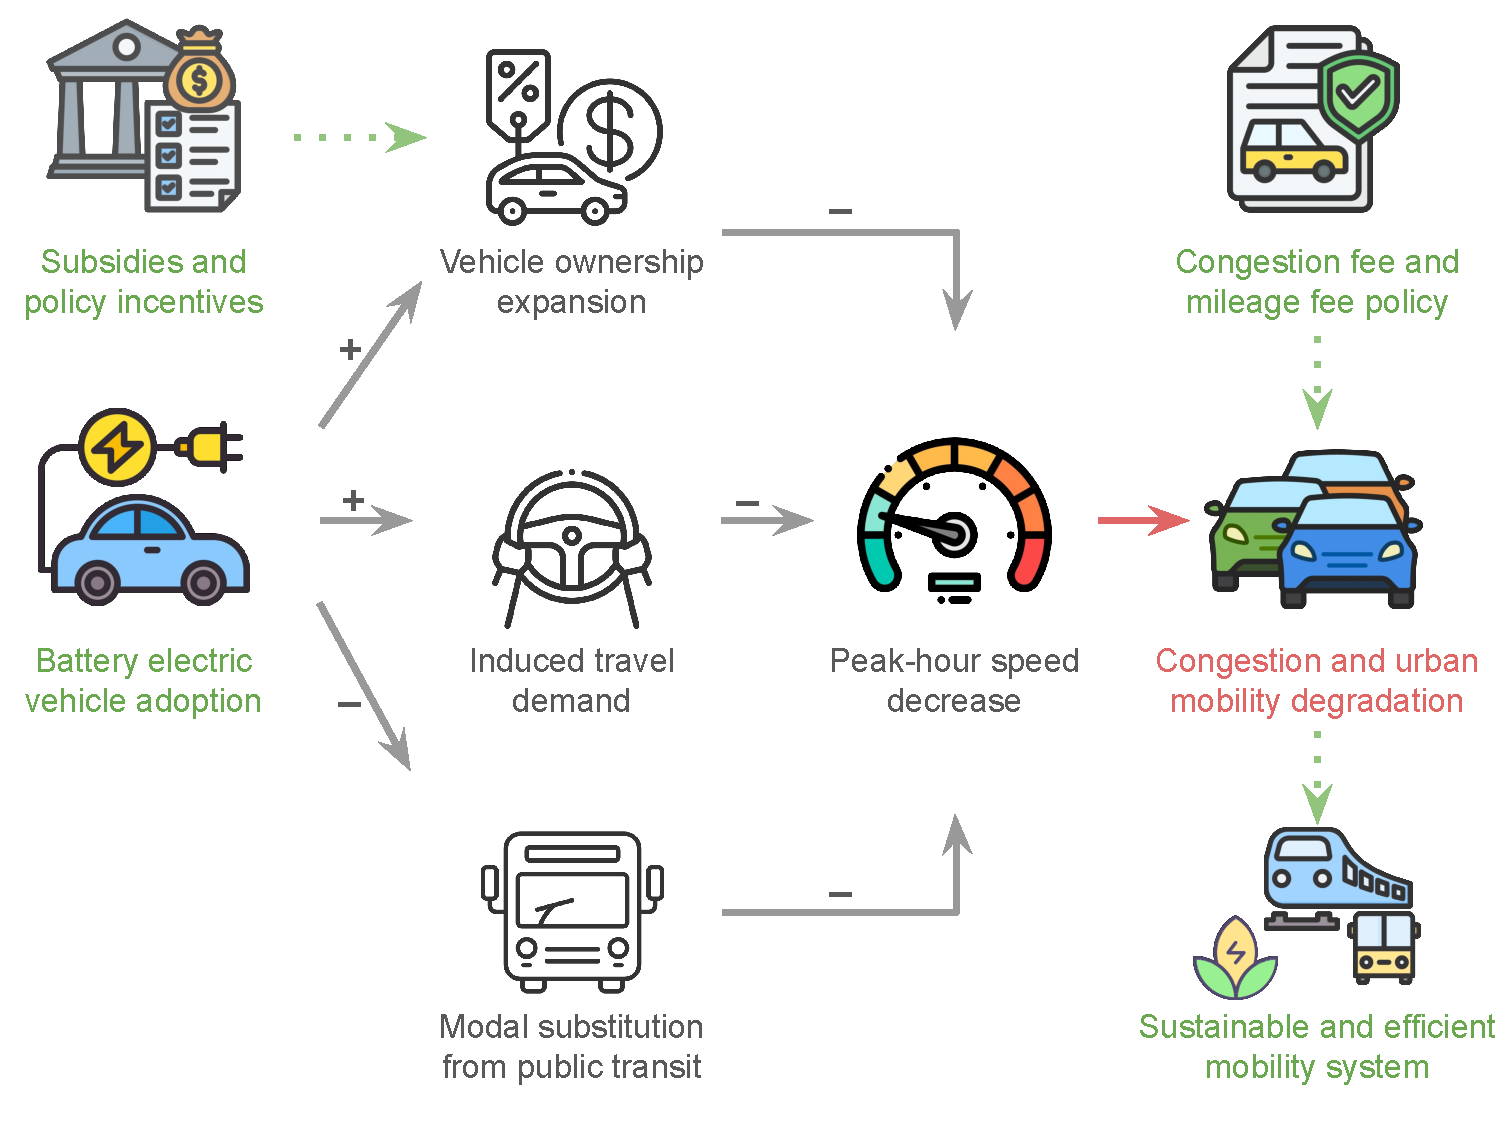
\includegraphics[width=0.8\textwidth]{flow_chart.pdf}
        \caption{\textbf{Conceptual framework linking the electric vehicle transition to traffic congestion.} Solid arrows indicate associations documented empirically in this study; dashed arrows indicate hypothesized pathways. Icons: Freepik, \url{flaticon.com}.}
    \label{fig:flow_chart}
\end{figure}

Beyond this average effect, we find substantial heterogeneity across community contexts.
The congestion effect is negative across most subgroups but amplified in communities with above-median income and population density, below-median transit commute shares, and above-median access to public charging infrastructure.
These patterns trace to distinct behavioral responses: vehicle ownership increases more sharply in high-income and high-density areas; low-transit communities experience both rising ownership and declining transit ridership; and charger-rich areas may introduce additional frictions, such as queuing and curbside congestion, that further degrade peak-hour speeds.
The two sides of the externality, moreover, fall on different communities.
Congestion costs concentrate where adoption concentrates, i.e., in affluent, dense, charger-rich areas whose drivers bear much of the added delay themselves.
The decline of public transit runs along the opposite gradient: ridership declines are largest in lower-income, car-dependent urbanized areas (Fig.~\ref{fig:heterogeneity-binned}D), where transit service is most fragile and where residents rely most on the alternatives that electrification undermines.
This two-sided pattern adds a spatial dimension to equity concerns in the transition to electric vehicles~\citep{Carlton2023, Hardman2021}: without complementary investments in transit alternatives and charging network design, the climate benefits of BEV adoption risk being paid for, in part, by communities already facing constrained transportation choices.

For policymakers, the lesson is that electrification policy should be paired with demand-management policy: BEVs mitigate GHG emissions and induce new travel demand at the same time~\citep{Jenn2018, Langbroek2016}, and ignoring the second margin erodes both the welfare and the emissions returns of the first through induced demand, fuel-tax revenue loss, and forgone fleet substitution.
To curb the induced demand from lower operating costs, state and local authorities could implement road-pricing mechanisms, such as congestion fees or mileage-based user fees, that apply equitably to all vehicles, including BEVs.
Such fees are widely discussed in the context of transportation finance~\citep{Noll2026, Levis2025}; our findings suggest they are also important to preserving the effectiveness of mitigation policy itself.
Purchase incentives could also be restructured to require, or at least encourage, the retirement of an existing ICE vehicle, preventing the expansion of multi-car household fleets; and public investment should prioritize transportation infrastructure in under-served neighborhoods so the transition does not deepen transportation inequities.
By shifting the policy focus from individual vehicle acquisition to total system efficiency, the electric transition can deliver a mobility future that is sustainable, efficient, and equitable.


\section{Conclusion}\label{sec:conclusion}
Using a decade of ZIP code-level registration records linked to statewide freeway sensor data, we find that BEV adoption in California is associated with increased traffic congestion, as measured by slower peak-hour freeway traffic, an effect that is absent at night and robust to regional shocks, the exclusion of pandemic years, alternative spatial definitions, and permutation inference.
The congestion effect is accompanied by fleet expansion, higher traffic flow, and lower transit ridership, and its costs fall unevenly across communities.
We argue that fleet electrification is a necessary part of transportation decarbonization, but on its own it does not address---and may aggravate---the congestion and car dependence that transportation policy has long aimed to reduce.
We suggest that pairing electrification with road pricing, incentives tied to vehicle retirement, and investment in under-served neighborhoods offers a path to capture its climate benefits while protecting the performance and equity of the transportation system.

This study has several limitations that offer directions for future research.
First, we assume static supply-side conditions and do not account for long-run equilibrium responses of urban planning and infrastructure development to the transition.
Second, while we identify a negative externality, we do not conduct a full welfare analysis; a comprehensive policy design would require weighing these congestion costs against the local air quality and global GHG benefits.
Third, we do not incorporate other emerging transportation technologies, such as transportation network companies and autonomous vehicles, which may reshape urban mobility systems.
Fourth, our traffic data are derived from the PeMS freeway sensor network, which covers freeways but not arterial roads.

\newpage
%% Declarations
\section*{Funding}
\noindent
This research did not receive any specific grant from funding agencies in the public, commercial, or not-for-profit sectors.

\section*{CRediT authorship contribution statement}
\noindent
\textbf{Ruoyu Chen:} Conceptualization, Data curation, Formal analysis, Methodology, Writing -- original draft, Writing -- review \& editing.
\textbf{Hang Liu:} Formal analysis, Methodology, Writing -- original draft.
\textbf{Mingzhi Zhou:} Conceptualization, Data curation, Writing -- original draft, Writing -- review \& editing.

\section*{Declaration of competing interest}
\noindent
The authors declare that they have no known competing financial interests or personal relationships that could have appeared to influence the work reported in this paper.

\section*{Acknowledgments}
\noindent
The authors thank Marlon Boarnet, Paulina Oliva, and Simon Quach for helpful feedback.
The authors thank conference participants at the annual meetings of the Transportation Research Board and the International Association for China Planning.

\section*{Data availability}
\noindent
The compiled ZIP code-level panel dataset and the code that reproduce all results in this study are available in a public GitHub repository (\url{https://github.com/ruoyuch/ev-congestion-public}).
All raw data are from publicly available sources: hourly freeway traffic data from the Caltrans Performance Measurement System (PeMS, \url{https://pems.dot.ca.gov}); ZIP code-level vehicle registration counts from the California Energy Commission (\url{https://www.energy.ca.gov/zevstats}); public transit ridership from the National Transit Database (\url{https://www.transit.dot.gov/ntd}); demographic and commuting controls from the American Community Survey (\url{https://www.census.gov/programs-surveys/acs/data.html}); public charging station data from the U.S. Department of Energy Alternative Fuels Data Center (\url{https://afdc.energy.gov/data_download}); and ZIP code-to-county and ZIP code-to-urbanized area crosswalks from the U.S. Department of Housing and Urban Development (\url{https://www.huduser.gov/portal/datasets/usps_crosswalk.html}), all accessed on 2 November 2026.


\section*{Declaration of AI-assisted technologies}
\noindent
During the preparation of this work, the authors used Claude (Anthropic) to assist with analytical code and language editing.
The authors reviewed and verified all outputs carefully and critically.

%% Reference
\newpage
\singlespacing\setlength\bibsep{0.5em}
\bibliography{references}
\setstretch{1.5}

%% Appendix
\newpage
\appendix
\section*{Appendix}
\setcounter{figure}{0}
\setcounter{table}{0}
\renewcommand{\thefigure}{A\arabic{figure}}
\renewcommand{\thetable}{A\arabic{table}}
\renewcommand{\theHfigure}{A\arabic{figure}}
\renewcommand{\theHtable}{A\arabic{table}}
\begin{figure}[H]
    \centering
    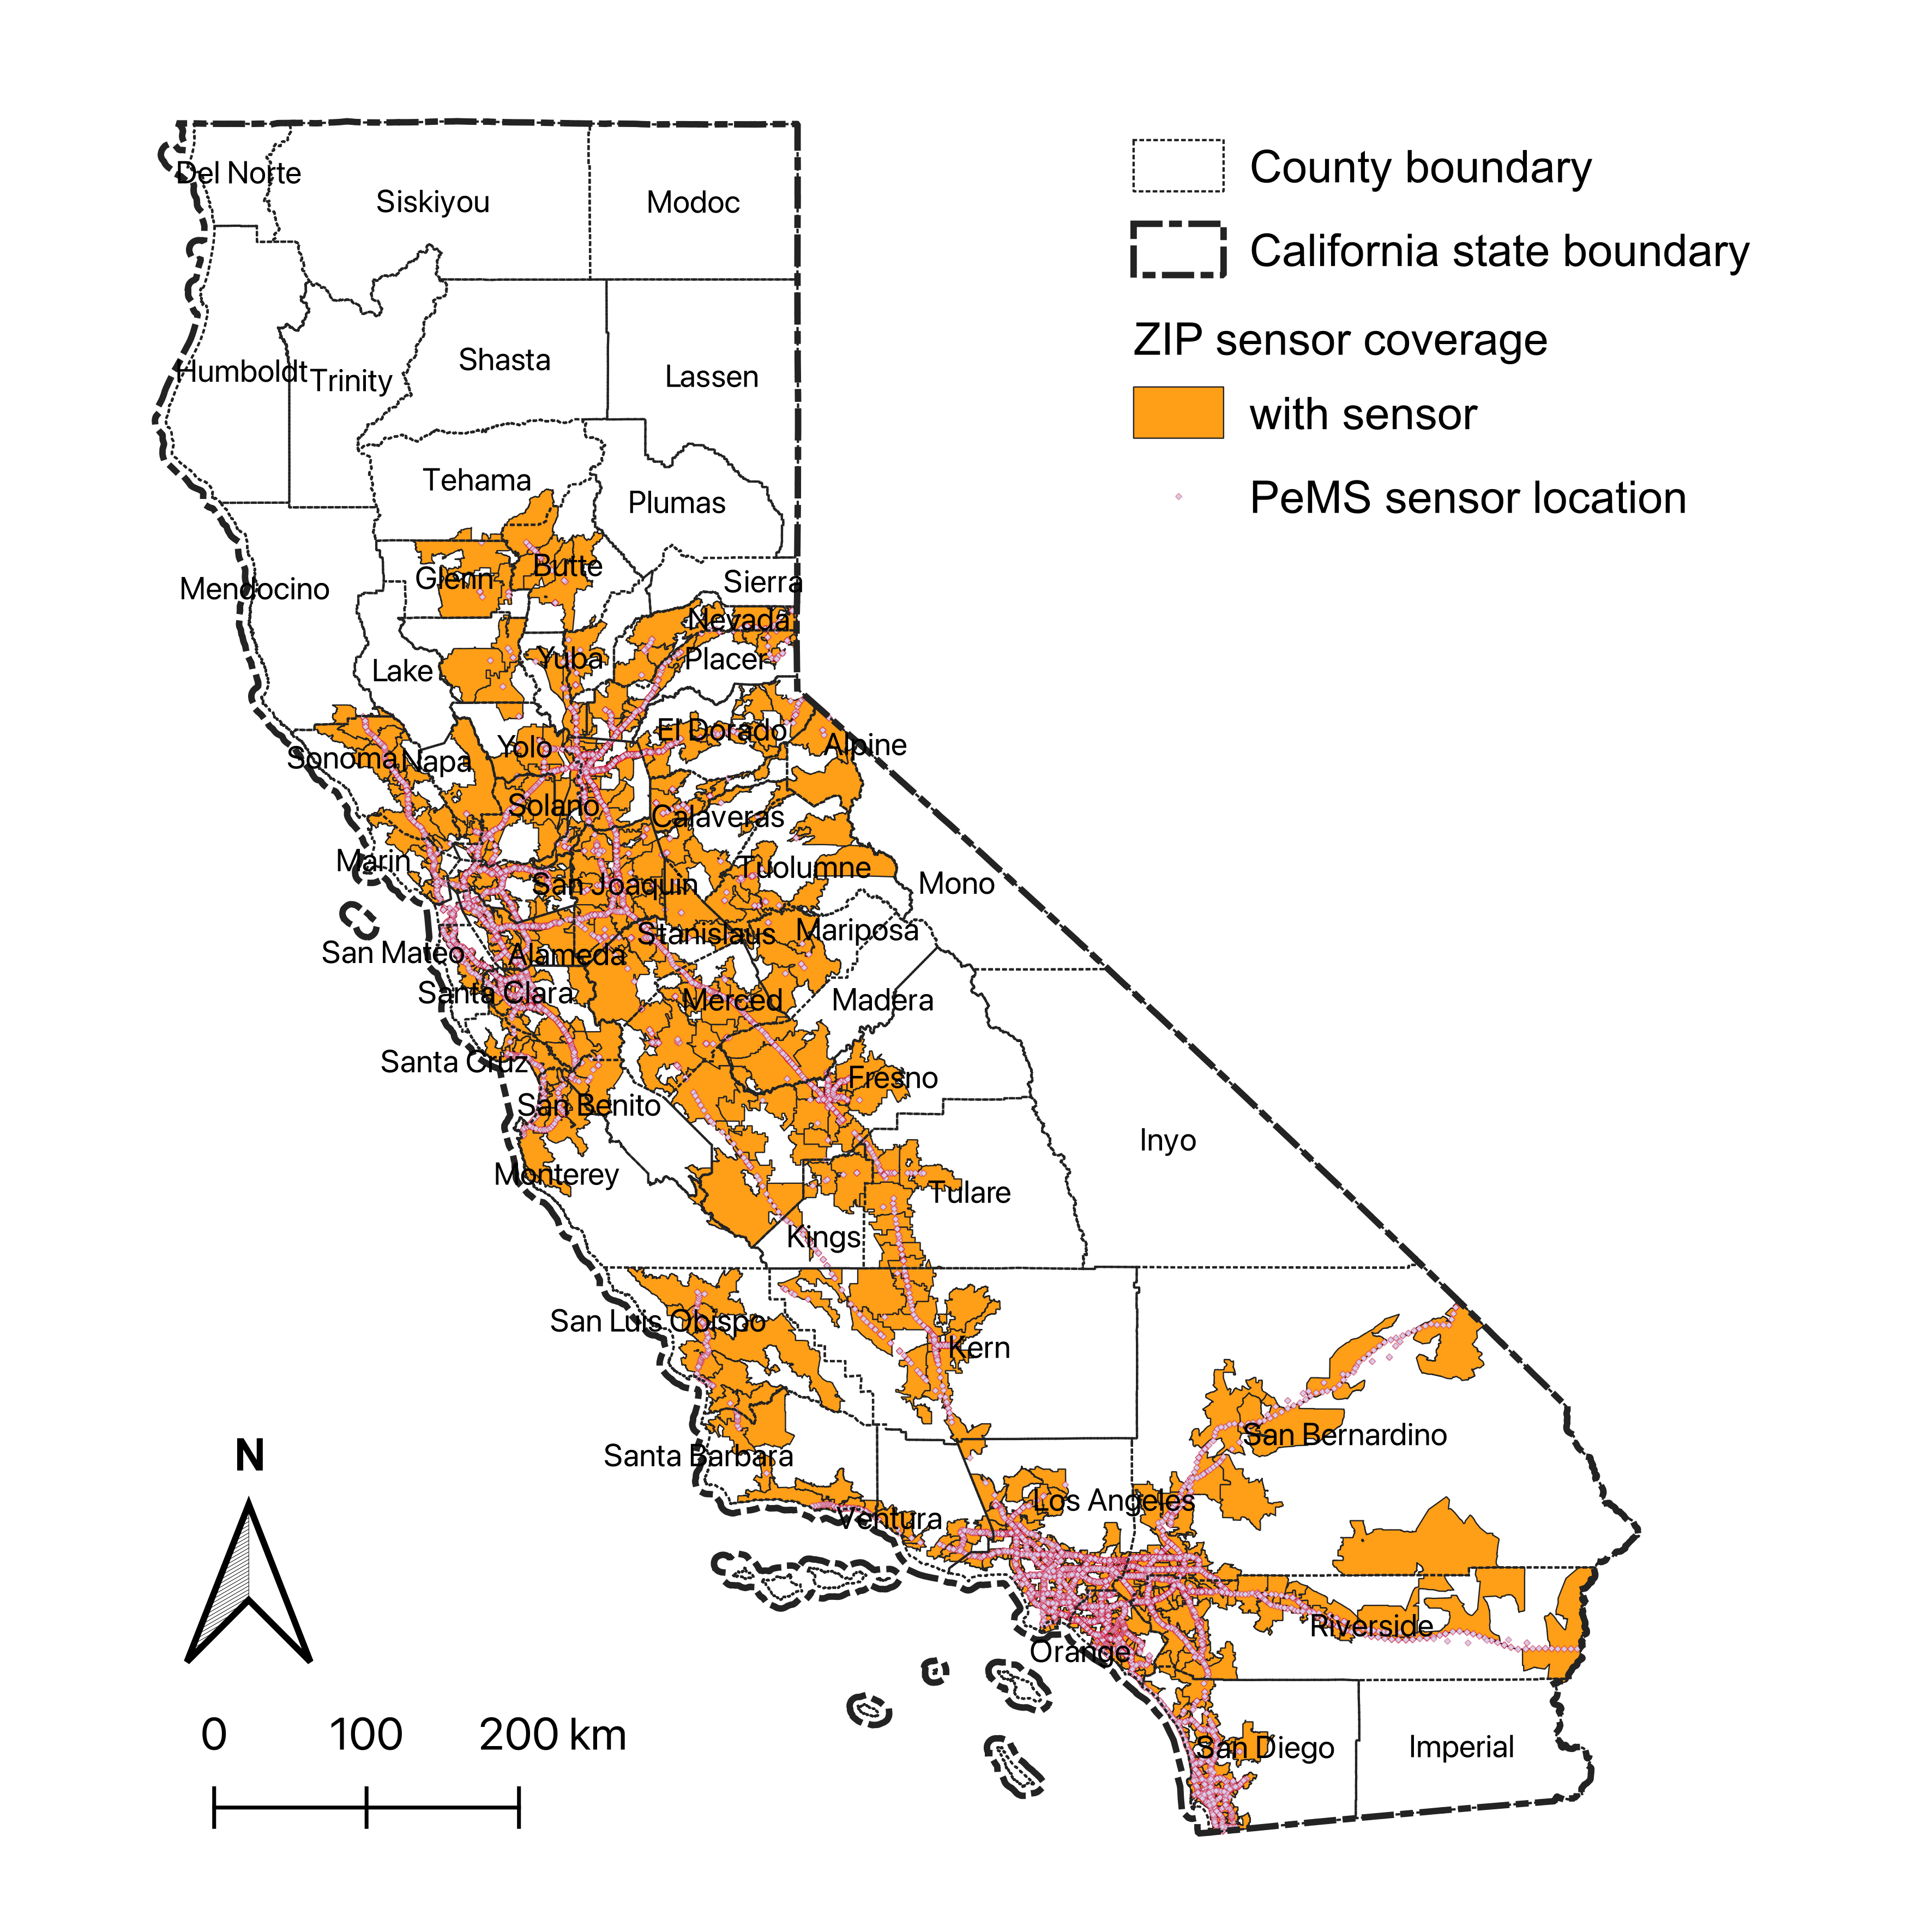
\includegraphics[width=0.6\textwidth]{map_pems_sensor.png}
    \caption{\textbf{Spatial coverage of Caltrans Performance Measurement System (PeMS) freeway sensors in California.} We use the traffic data from the sensors to calculate our primary outcome variable in the study. The map shows that the dataset covers the majority of populated areas in California.}
    \label{fig:pems-sensor-map}
\end{figure}

\newpage
\begin{figure}[H]
    \centering
    \includegraphics[width=0.65\textwidth]{../output/figures/cvrp_bin_es_fs.pdf}
    \caption{\textbf{Event study of the CVRP income-eligibility reform on BEV adoption.} Coefficients on interactions between the pre-reform ZIP-level share of households with annual income above \$100,000 and indicators for years relative to 2017, the first full year under the Clean Vehicle Rebate Project (CVRP) income caps, from a regression of log battery electric vehicle (BEV) count with ZIP code and year fixed effects and the full set of controls, California, 2014--2023. The reference year is 2016. Error bars show 95\% confidence intervals based on standard errors clustered by ZIP code.}
    \label{fig:event-study-iv}
\end{figure}

\newpage
\begin{figure}[H]
    \centering
    \includegraphics[width=0.7\textwidth]{../output/figures/permutation_test.pdf}
    \caption{\textbf{Permutation test of the baseline estimate.} Battery electric vehicle (BEV) adoption trajectories are randomly reassigned across ZIP codes 1,000 times and the baseline two-way fixed effects model is re-estimated on each permuted sample. The histogram shows the resulting placebo coefficients; the vertical line marks the actual estimate ($-0.0099$).}
    \label{fig:permutation-test}
\end{figure}

\newpage
\begin{figure}[H]
    \centering

    % Panel (A)
    \begin{minipage}[t]{0.48\textwidth}
        \centering
        \footnotesize (A) Excluding one year at a time\\[4pt]
        \includegraphics[width=\textwidth]{../output/figures/loo_year.pdf}
    \end{minipage}
    \hfill
    % Panel (B)
    \begin{minipage}[t]{0.48\textwidth}
        \centering
        \footnotesize (B) Excluding one county at a time\\[4pt]
        \includegraphics[width=\textwidth]{../output/figures/loo_county.pdf}
    \end{minipage}

    \caption{\textbf{Leave-one-out robustness of the baseline estimate.} Each point re-estimates the baseline two-way fixed effects model of log weekday peak-hour freeway speed on log battery electric vehicle count, excluding (\textbf{A}) one year or (\textbf{B}) one county at a time. Dashed lines mark the full-sample estimate; error bars indicate 95\% confidence intervals.}
    \label{fig:loo-checks}
\end{figure}

\newpage
\begin{table} [H]
    \centering
    \caption{\small \textbf{First stage of the instrumental variable design.}}
    \begin{footnotesize}
        \input{../output/tables/cvrp_iv_table.tex}
    \end{footnotesize}
    \label{tab:first-stage-iv}
\end{table}

\newpage
\begin{table} [H]
    \centering
    \caption{\small \textbf{Effects of lagged BEV adoption on traffic congestion.}}
    \begin{footnotesize}
        \input{../output/tables/twfe_speed_regs_lag.tex}
    \end{footnotesize}
    \label{tab:twfe-speed-regs-lag}
\end{table}

\newpage
\begin{table} [H]
    \centering
    \caption{\small \textbf{Effects of BEV adoption measured at alternative distance bands.}}
    \begin{footnotesize}
        \input{../output/tables/donut_regs.tex}
    \end{footnotesize}
    \label{tab:donut-regs}
\end{table}

\newpage
\begin{table} [H]
    \centering
    \caption{\small \textbf{Robustness to excluding COVID-19-affected years.}}
    \begin{footnotesize}
        \input{../output/tables/twfe_speed_regs_covid.tex}
    \end{footnotesize}
    \label{tab:twfe-speed-regs-covid}
\end{table}

\newpage
\begin{table} [H]
    \centering
    \caption{\small \textbf{Robustness to regional shocks, trends, and pandemic years.}}
    \begin{footnotesize}
        \textbf{Panel A. Peak-hour speed}\\[0.5ex]
        \input{../output/tables/twfe_speed_regs_robust_peak.tex}
        \\[2ex]
        \textbf{Panel B. Midnight speed (placebo)}\\[0.5ex]
        \input{../output/tables/twfe_speed_regs_robust_mn.tex}
    \end{footnotesize}
    \label{tab:twfe-speed-regs-robust}
\end{table}

\end{document}
